\begin{figure}[!hb]
  \centering
  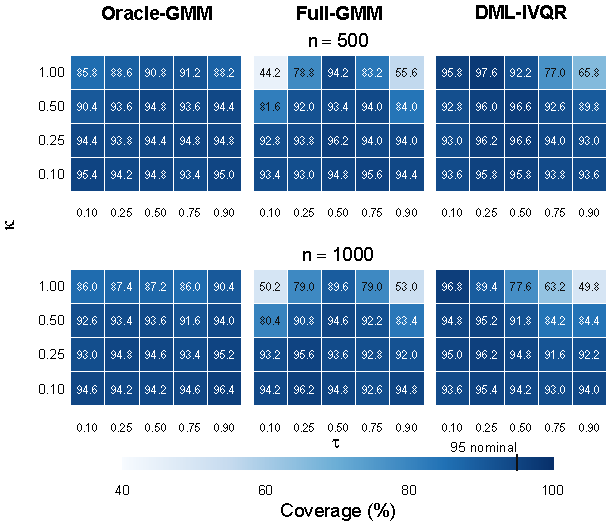
\includegraphics[width=0.72\textwidth]{figures/generated/coverage_heatmap.pdf}
  \caption{Empirical coverage across simulation designs.}
  \label{fig:coverage-heatmap}
  \begin{figurenotes}
    Nominal coverage is 95\%; each cell uses 500 complete replications. Coverage is the fraction of tests accepting the true parameter, evaluated directly at that parameter rather than reconstructed from grid membership. Panel columns identify estimators; panel rows show $n=500$ and $n=1000$. Within each panel, columns show quantiles $\tau$ and rows show relevance $\kappa$, declining from 1.00 to 0.10. Annotations and the common colour scale report percentages. Darker shading indicates higher coverage, not necessarily better calibration.
  \end{figurenotes}
\end{figure}
